\documentclass{article}
\usepackage{arxiv}
\usepackage[utf8]{inputenc} % allow utf-8 input
\usepackage[T1]{fontenc}    % use 8-bit T1 fonts
\usepackage{hyperref}       % hyperlinks
\usepackage{url}            % simple URL typesetting
\usepackage{booktabs}       % professional-quality tables
\usepackage{amsfonts}       % blackboard math symbols
\usepackage{nicefrac}       % compact symbols for 1/2, etc.
\usepackage{microtype}      % microtypography
\usepackage{lipsum}
\usepackage{amsthm}
\usepackage{amsmath}
\usepackage{minted}
\usepackage{graphicx}
\usepackage{caption}

\newtheorem{theorem}{Theorem}
\newtheorem{lem}[theorem]{Lemma}
\newtheorem{proposition}[theorem]{Proposition}
\theoremstyle{definition}
\newtheorem{definition}[theorem]{Definition}

\title{Research project}

\examineenumber{11070}
\author{Gábor Ádám Fehér}

\begin{document}
\maketitle

\newpage

\section*{Answer to Theme A}
From the fundamental concepts related to mathematical informatics we present the \textbf{Cooley–Tukey algorithm}. The algorithm allows us to compute the discrete Fourier transform of a \(n\) long sequence in \(\mathcal{O}(n\log{}n)\) time. Algorithm with such properties are called fast Fourier transform (FFT) algorithms. Among the many variants of the Cooley–Tukey algorithm, the \textbf{radix-2 DIT} is the simplest and most common one, and thus we present it in great detail. Other forms of the algorithm, as well as other types of FFT algorithms, are also mentioned but no rigorous construction is given.

\subsection*{Mathematical overview}
\begin{definition}[Discrete Fourier transform]
    The discrete Fourier transform (DFT) over the \(n\) dimensional complex field is an invertible linear transformation \(\mathcal{F}: \mathbb{C}^n \to \mathbb{C}^n\). The output of the function for \({(x_k)}_{0 \leq k \leq n - 1}\) is defined by
    \begin{gather}
        X_k = \left(\mathcal{F}(x)\right)_k = \sum_{j=0}^{n-1} x_j e^{-\frac{2{\pi}ikj}{n}} =  \sum_{j=0}^{n-1} x_j \left[ \cos\left( \frac{2{\pi}ikj}{n} \right) - i \sin\left( \frac{2{\pi}ikj}{n} \right) \right],
    \end{gather}
    where the right side of the equation is due to Euler's formula and the trigonometric properties of sine and cosine.
\end{definition}

We should mention that the sign of the exponential is sometimes taken as positive. The resulting equation is equal to the inverse of the previously defined Fourier transformation multiplied by the constant \(n\), that is
\begin{gather}
    x_k = \left(\mathcal{F}^{-1}(X)\right)_k = \frac{1}{n}\sum_{j=0}^{n-1}X_j e^{\frac{2{\pi}ikj}{n}}.
\end{gather}
With some minor adjustments the Cooley–Tukey algorithm is capable of computing the inverse-DFT of the \(n\) long sequence, so no matter which convention we use, the algorithm remains useful.

We introduce some notations. Given \(x = (x_k)_{0 \leq 2n-1}\), we define \(X^{[0]}\) to be the DFT of the even-indexed terms, while \(X^{[1]}\) to be the DFT of the odd-indexed terms in the sequence. That is
\begin{gather}
    X^{[0]}_k = \left(X^{[0]}\right)_k = \left(\mathcal{F}(x_0, x_2, \dots x_{2n-2})\right)_k = \sum_{j=0}^{n-1} x_{(2j)} e^{-\frac{2{\pi}ikj}{n}} = \sum_{j=0}^{n-1} x_{(2j)} e^{-\frac{4{\pi}ikj}{2n}} \label{dq:1} \\
    X^{[1]}_k = \left(X^{[1]}\right)_k = \left(\mathcal{F}(x_1, x_3, \dots x_{2n-1})\right)_k = \sum_{j=0}^{n-1} x_{(2j+1)} e^{-\frac{2{\pi}ikj}{n}} = \sum_{j=0}^{n-1} x_{(2j+1)} e^{-\frac{4{\pi}ikj}{2n}}. \label{dq:2}
\end{gather}
The key observation to make in order to verify the validity of the algorithm is
\begin{gather}
    X_k = \sum_{j=0}^{2n-1} x_j e^{-\frac{2{\pi}ikj}{2n}} = \sum_{j=0}^{n-1} x_{(2j)} e^{-\frac{4{\pi}ikj}{2n}} + e^{-\frac{2{\pi}ik}{2n}}\sum_{j=0}^{n-1} x_{(2j+1)} e^{-\frac{4{\pi}ikj}{2n}}. \label{dq:4}
\end{gather}
Thus for \(0 \leq l \leq n-1\) we have
\begin{gather}
    X_l = X^{[0]}_l + e^{-\frac{2{\pi}ik}{2n}} X^{[1]}_l, \text{ and }
    X_{n+l} = X^{[0]}_l - e^{-\frac{2{\pi}ik}{2n}} X^{[1]}_l, \label{dq:3}
\end{gather}
since
\begin{gather}
    \sum_{j=0}^{n-1} x_{(2j)} e^{-\frac{4{\pi}i(n+l)j}{2n}} = \sum_{j=0}^{n-1} x_{(2j)} e^{-\frac{4{\pi}ilj}{2n}}, \text{ and } e^{-\frac{2{\pi}i(n+l)}{2n}} = -e^{-\frac{2{\pi}il}{2n}}.
\end{gather}

\subsection*{The algorithm}
This basis of all variants of the Cooley–Tukey algorithm is the divide-and-conquer technique. In the radix-2 case the size of the input has to be a power of two. We may add padding zeros to fit the size constraint. From this point on we assume that input vectors are of the right size. Given an \({x}_{0\leq k \leq n}\), where \(2\leq n\), equations \ref{dq:1} and \ref{dq:2} indicate that the input vector should be divided into two parts: the even-indexed and the odd-indexed terms. Once the DFTs of the split vector are calculated, via recursive calls, the DFT of the input vector can be calculated by using equation \ref{dq:3}. If the input vector is one dimensional, its DFT is itself. The following Python code is a working implementation of the radix-2 case, illustrating the key ideas used, but due to its performance it is not meant to be used in real world applications.
\inputminted[xleftmargin=20pt, linenos]{python}{./code/recursive_fft.py}
To evaluate the time complexity of the algorithm, apart from the recursive calls in line 13 and 14, the algorithm runs in \(\Theta(n)\) time, where \(n\) is the length of the input. Using the recurrence relation
\begin{gather}
    T(n) = 2T(n/2) + \Theta(n) = \Theta(n\log{}n).
\end{gather}
With little modification, the Cooley–Tukey algorithm can compute the inverse-DFT of a transformed vector. Similarly to equation \ref{dq:4}, we can derive
\begin{gather}
    x_k = \sum_{j=0}^{2n-1} X_j e^{\frac{2{\pi}ikj}{2n}} = \sum_{j=0}^{n-1} X_{(2j)} e^{\frac{4{\pi}ikj}{2n}} + e^{\frac{2{\pi}ik}{2n}}\sum_{j=0}^{n-1} X_{(2j+1)} e^{\frac{4{\pi}ikj}{2n}}
\end{gather}
so in the 9th line, instead of \(e^{-2{\pi}i/N}\) we have \(e^{2{\pi}i/N}\) for the \(N\) long input, and by multiplying each term of the end result by \(1/n\) given the initial input had size of \(n\), we obtain the original \(x\), within the same time complexity.
\subsection*{Importance and Usage}
The FFT is widely used among different fields of engineering, computer science and mathematics. 

Many popular compression methods, such as \texttt{jpeg} or \texttt{webm}, use discrete cosine transforms (DCT). Algorithms that compute DCTs in \(\mathcal{O}(n\log{}n)\) are known as fast cosine transform (FCT) algorithms. Specialized FCT algorithms exist, that directly compute a vectors DCT, and tough the theoretical running time of such algorithms are better, on modern hardware computing DCTs via FFTs with some \(\mathcal{O}(n)\) pre- and post-processing steps are often faster.

When two degree-bound \(n\) polynomials are represented in the a "extended" point-value form, over \(2n\) distinct points, multiplication can be done in \(\mathcal{O}(n)\) time, by simply multiplying the coefficients. Representing such a polynomial over the \(n\)th root of unity is the same as having the coefficient vectors transformed. Thus multiplying two polynomials can be done in \(\mathcal{O}(n\log{}n)\) time by using FFTs: first transforming the polynomials to their "extended" point value form in \(\mathcal{O}(n\log{}n)\) time, multiplying them in \(\mathcal{O}(n)\), and then transforming back the result to coefficient form. Polynomial representation of the Toeplitz matrices also allow us to multiply them within the same time complexity.

FFts are also widely used in theoretical results. For a long time the \textbf{Schönhage–Strassen algorithm} was the fastest known algorithm for multiplying two large integers. With running time \(\mathcal{O}(n\log{}n\log{}\log{}n)\), it is asymptotically faster than other many traditional multiplication methods, like for example the \textbf{Karatsuba algorithm}, but it only starts to outperform them for numbers with 10000 to 40000 digits, thus it is rarely used in practice. The algorithm employs modular arithmetic instead of the roots of unity (Fourier transforms can be performed in any algebric ring). In 2019 Harvey and van der Hoeven published a \(\mathcal{O}(n\log{}n)\) algorithm, which also builds upon on FFTs. However this is a galactic algorithm, so it only bears theoretical importance.

\section*{Answer to Theme B}
\newpage
\section*{Answer to Theme C}
Mathematical informatics can help immensely to prepare for and to handle infectious diseases. After a brief introduction to the subject, we introduce methodologies to combat each stages of an epidemic. We also take into consideration the recent case of COVID-19, and what are the protective measures that can be implemented and its effects. We should also mention that in the case of an outbreak, the tools of bioinformatics are a useful to analyse the pathogens properties and to develop vaccines but we choose to focus on analytical methods to make precautionary decisions and combat its spread.

\subsection*{Basic concepts}
Compartment models are widely used in modeling infectious diseases. In case of an outbreak, each member of the population is assigned with a label, depending on the individuals relation with the infectious agent. An example would be the labels \textbf{S} for susceptible, \textbf{I} for infectious and \textbf{R} for recovered/removed. Individuals with the same label form a compartment. Individuals may also progress between compartments. The underlying social structure may taken to be homogenous, or can me modeled with small-world networks. Models most use differential equations to simulate the movement of people between different compartments, but stochastic frameworks have also been introduced. 

Generally epidemic containment efforts have four phases: \textbf{preparedness}, \textbf{outbreak investigation}, \textbf{response} and \textbf{evaluation}. These phases contain a wide range of tasks, such as inventory management for essential medical supply and network design for transportation activities during the preparation phase, surveillance system design and implementation during the investigation phase, selection of facilities as PODs (Point of Dispensing) and scheduling of vehicles to be used for transportation during the response phase and identification of bottlenecks during the evaluation phase. Even tough being well prepared is essential, the uncertainties present at an epidemic outbreak dictate the use of real-time solutions. In such an event, decision-makers have to be presented with a wide range of models, that forecast how the epidemic will play out. In the subsequent sections we focus on two key issues they face, the diffusion of the epidemic and the distribution of emergency resources based on demand.

\subsection*{Epidemic modelling}
Different scenarios dictate the use of different models to forecast the diffusion of the infectious agent. These properties may be due to the nature of of the infectious agent or the policy to be implemented. For example if the agent has incubation time, the appropriate compartment needs to be included in the model. The use of quarantine also creates an additional compartment in the model, but this aspect of the model can be controlled by the acting official. Travel and migration is another aspect which can be controlled. The following diagram showcases the model which describes the model many countries have implemented in the wake of the COVID-19 outbreak.
\begin{figure}[H]
    \centering
    \def\svgwidth{0.7\columnwidth}
    \input{./figures/model_seiqr.pdf_tex}
    \captionsetup{justification=centering,margin=2cm}
    \caption{SEIQRS model}
\end{figure}
% 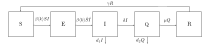
\includepdf[pages=-]{figures/model_seiqr.pdf}

\bibliographystyle{unsrt}
% \begin{thebibliography}{1}

%   \bibitem{basek2013}
%   Gopal Basak and Stanislav Volkov.
%   \newblock Snakes and perturbed random walks
%   \newblock In {\em Proceedings of the Steklov Institute of Mathematics, vol 282, no. 1}, pages. 35--44. Springer, 2013

% \end{thebibliography}
\end{document}